% 1985 广东理工农医类第一卷二（1）：原卷 A–E 五个函数图示，曲线只表达形状。
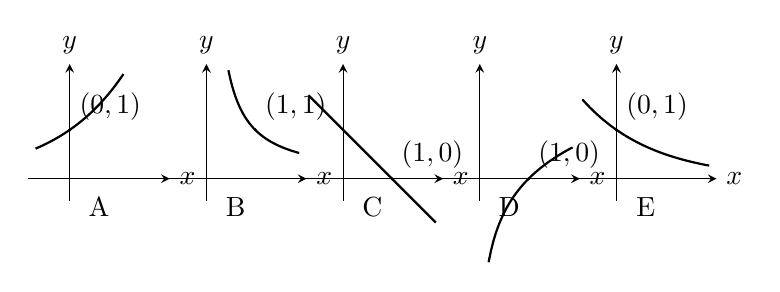
\begin{tikzpicture}[scale=0.62,>=stealth]
  \foreach \x/\label in {0/A,2.8/B,5.6/C,8.4/D,11.2/E} {
    \begin{scope}[shift={(\x,0)}]
      \draw[->] (-0.85,0)--(2.05,0) node[right] {$x$};
      \draw[->] (0,-0.45)--(0,2.35) node[above] {$y$};
      \node at (0.6,-0.58) {\label};
    \end{scope}
  }
  % A 递增，过 (0,1)
  \begin{scope}
    \draw[thick,domain=-0.7:1.1,samples=35] plot (\x,{2^\x});
    \fill (0,1) circle (1pt) node[above right] {$(0,1)$};
  \end{scope}
  % B 递减，标 (1,1)
  \begin{scope}[shift={(2.8,0)}]
    \draw[thick,domain=0.45:1.9,samples=35] plot (\x,{1/\x});
    \fill (1,1) circle (1pt) node[above right] {$(1,1)$};
  \end{scope}
  % C 递减，穿过 (1,0)
  \begin{scope}[shift={(5.6,0)}]
    \draw[thick,domain=-0.7:1.9,samples=35] plot (\x,{1-\x});
    \fill (1,0) circle (1pt) node[above right] {$(1,0)$};
  \end{scope}
  % D 递增，穿过 (1,0)
  \begin{scope}[shift={(8.4,0)}]
    \draw[thick,domain=0.18:1.9,samples=35] plot (\x,{ln(\x)});
    \fill (1,0) circle (1pt) node[above right] {$(1,0)$};
  \end{scope}
  % E 递减指数曲线，过 (0,1)
  \begin{scope}[shift={(11.2,0)}]
    \draw[thick,domain=-0.7:1.9,samples=35] plot (\x,{2^(-\x)});
    \fill (0,1) circle (1pt) node[above right] {$(0,1)$};
  \end{scope}
\end{tikzpicture}
